%use scrbook and set dotted line
\documentclass[toc=chapterentrywithdots,openany]{scrbook}
%use a4paper for a4 paper and size 
\usepackage[a4paper,left=30mm,right=30mm,top=30mm, bottom=30mm]{geometry}
%use german
\usepackage{german}
%silence a not relevant warning
%https://tex.stackexchange.com/questions/349473/suppress-warning-usage-of-package-fancyhdr-togetherscrbook-with-a-koma-scr
\usepackage{silence}
\WarningFilter{scrbook}{Usage of package `fancyhdr'}

%use colorpackage to set font colors
\usepackage{xcolor}
%use fancyhdr to set the header
\usepackage{fancyhdr}
%use helvetica font
\usepackage[]{helvet}
%use tocbibind to see the toc in the toc
\usepackage{tocbibind}
%user hyperref to add links
\usepackage{hyperref}
%use graphicx to add images
\usepackage{graphicx}
%path for the images
\graphicspath{ {figures/} }
%renewcommand to apply the font
\renewcommand\familydefault{\sfdefault}

%use graphicx to add images
\usepackage{graphicx}

%use inputenc to set the encoding
\usepackage[utf8]{inputenc}


%start the document
\begin{document}

%titlepage
%variableto fill
\newcommand{\Thema}{Mein Thema}
\newcommand{\Name}{Vorname nachname}
\newcommand{\Gutachter}{Dr. Herbert Bauer}
\newcommand{\Matrikelnummer}{123456}
\newcommand{\Abgabedatum}{09.01.2022}




\begin{titlepage}
	\newgeometry{left=2cm, right=2cm, top=2cm, bottom=2cm}
	%center the logo and display the FOM graphic
	\begin{center}
		
\includegraphics[width=2.3cm]{assets/fomLogo.pdf}\\
		\vspace{.5cm}
		%strong text
		\begin{Large}\textbf{FOM Hochschule für Ökonomie und Management}\end{Large}\\
		\vspace{.5cm}
		Hochschulzentrum München

		\vspace{2cm}
	\end{center}

	%create big space
	\bigskip

	\begin{center}
		%bold text
		\textbf{Seminararbeit}\\
		\vspace{0.2cm}
		Im Rahmen des Moduls\\
		\vspace{0.5cm}
		Arbeitsmethoden und Softwareunterstützung\\
		\vspace{2cm}
		Über das Thema\\
		\vspace{0.5cm}
		%bold text
		\begin{Large}\textbf{\textbf{\Thema}}\end{Large}\\

		\vspace{2cm}
		von\\
		\vspace{0.5cm}
		\begin{Large}\textbf{\textbf{\Name}}\end{Large}\\
	\end{center}

	%postion in bottom left
	\begin{figure}[b]

		Gutachter: \Gutachter       \\
		Matrikelnummer: \Matrikelnummer \\
		Abgabedatum: \Abgabedatum
	\end{figure}

\end{titlepage}

%pagenumbering
\fancypagestyle{plain}{%
	\fancyhf{} % clear all header and footer fields
	\fancyhead{} % clear all header fields
	\fancyfoot{} % clear all footer fields
	\fancyhead[C]{\textcolor{gray}\thepage} 
	\renewcommand{\headrulewidth}{0pt}
	\renewcommand{\footrulewidth}{0pt}
}
%use roman for the page number
\pagenumbering{Roman}
%set the toc to 2
\setcounter{page}{2}


%inhaltsverzeichnis
hallo
%abbildungen
\listoffigures
\listoftables
%tabellen
%symbole und formeln
\input{formel-symbolverzeichnis}

\newpage

%reset pagestyle to continue with arabic numbering
\pagestyle{plain}
%pagenumbering
\fancypagestyle{plain}{%
	\fancyhf{} % clear all header and footer fields
	\fancyhead{} % clear all header fields
	\fancyfoot{} % clear all footer fields
	\fancyhead[C]{\textcolor{gray}\thepage}
	\renewcommand{\headrulewidth}{0pt}
	\renewcommand{\footrulewidth}{0pt}
}
\pagenumbering{arabic}

\chapter{Einleitung der Arbeit}

\section{Forschungsfrage}

Welche Auswirkungen haben Kraftfahrzeuge auf die Umwelt und wie kann autonomes Fahren die negativen Auswirkungen reduzieren?

\section{Hypothese}

Je mehr Fahrzeuge autonom fahren, desto geringer fällt die Feinstaubbelastung durch Kfz aus.



\section{TBD}

-Kraftfahrzeuge einfluss auf die Umwelt
-steigende Zulassung bei Fahrzeugen durch steigende Globalisierung
-steigende Temperaturen, Feinstaubbelastung
-steigende CO2-Emissionen durch Kfz
-durch bessere Fertigungsmethoden gibt es mehr Autos
-Umweltbelastung durch Umwege
-Umweltbelastung durch Fahrfehler
-Umweltbelastung durch Kfz-Fahrer
-Umweltbelastung durch Staus
-Umweltbelastung durch LKW

\section{Definitionen}
\subsection{Kraftfahrzeuge}

\textit{Als Kraftfahrzeuge im Sinne dieses Gesetzes gelten Landfahrzeuge, die durch Maschinenkraft bewegt werden, ohne an Bahngleise gebunden zu sein.}
\footnote{Straßenverkehrsgesetz, § 1 Abs. 2}
\vspace{0.5cm}
\newline
Kraftfahrzeuge können in folgende Kategorien eingeteilt werden\footnote{VERORDNUNG (EU) Nr. 678/2011 DER KOMMISSION
	vom 14. Juli 2011, TEIL A ABS.1 - https://eur-lex.europa.eu/eli/reg/2011/678/oj?locale=de}:
\begin{itemize}
	\item Klasse M (Vorwiegend für die Beförderung von Fahrgästen und deren Gepäck ausgelegte und gebaute Kraftfahrzeuge)
	\item Klasse N (Vorwiegend für die Beförderung von Gütern ausgelegte und gebaute Kraftfahrzeuge.)
	\item Klasse O (Anhänger, die sowohl für die Beförderung von Gütern und Fahrgästen als auch für die Unterbringung von Personen ausgelegt und gebaut sind.)
	\item Klasse S (unvollständige Fahrzeuge, die der Unterklasse der Fahrzeuge mit besonderer Zweckbestimmung zugeordnet werden soll)
\end{itemize}


\subsection{Autonomes Fahren}

Beim autonomen Fahren, fährt ein \ac{Kfz} verwaltungsgemäß selbständig.
Für \ac{Kfz} wurden von der \ac{SAE} Institut in der Norm SAE J3016\footnote{SAE J3016\textunderscore202104 - https://www.sae.org/standards/content/j3016\textunderscore202104} Automatisierungsgrade definiert.
\begin{itemize}
	\item Stufe 0 (Keine Automation)
	\item Stufe 1 (Assistenzsysteme)
	\item Stufe 2 (Teilautomatisierung)
	\item Stufe 3 (Bedingte Automatisierung)
	\item Stufe 4 (Hochautomatisierung)
	\item Stufe 5 (Vollautomatisierung)
\end{itemize}
\subsubsection{Was passiert in den Stufen?}
In der Stufe 0 (Keine Automation):
\begin{itemize}
	\item keine Assistenzsysteme
	\item \ac{Kfz} kann keine Fahraufgaben übernehmen
	\item Fahrer ist unter permanenter Kontrolle
\end{itemize}

In der Stufe 1 (Assistenzsysteme):
\begin{itemize}
	\item Assistenzsysteme wie Geschwindigkeitsregelanlage oder eine Berganfahrhilfe
	\item Fahrer hat eine passive Unterstützung bei Fahraufgaben
	\item \ac{Kfz} kann keine Fahraufgaben übernehmen
	\item Fahrer ist unter permanenter Kontrolle
\end{itemize}

In der Stufe 2 (Teilautomatisierung):
\begin{itemize}
	\item Assistenzsysteme, wie der Spurführungsassistent oder Stauassistent
	      \begin{itemize}
		      \item automatisch bremsen
		      \item automatisch beschleunigen
		      \item automatisch lenken
	      \end{itemize}
	\item \ac{Kfz} kann Fahraufgaben teilautomatisiert übernehmen
	\item Fahrer kann sich für kurze Zeit von den Fahraufgaben abwenden
	\item Fahrer muss jeder Zeit die Fahraufgabe übernehmen können
\end{itemize}

In der Stufe 3 (Bedingte Automatisierung):
\begin{itemize}
	\item hochautomatisierte Assistenzsysteme
	\item \ac{Kfz} kann Fahraufgaben unter bestimmten Voraussetzungen vollständig übernehmen
	\item Fahrer kann sich unter bestimmten Voraussetzungen dauerhaft von den Fahraufgaben abwenden
	\item Fahrer muss innerhalb wenigen Sekunden die Fahraufgabe übernehmen können
\end{itemize}

In der Stufe 4 (Hochautomatisierung):
\begin{itemize}
	\item hochautomatisierte Assistenzsysteme
	\item \ac{Kfz} kann Fahraufgaben in hochkomplexen Verkehrssituationen vollständig übernehmen
	\item Fahrer dauerhaft von den Fahraufgaben abwenden
	\item Fahrer muss fahrtüchtig sein, um im Bedarfsfall die Fahraufgabe übernehmen zu können
\end{itemize}

In der Stufe 5 (Vollautomatisierung):
\begin{itemize}
	\item hochautomatisierte Assistenzsysteme
	\item \ac{Kfz} übernimmt alle Fahraufgaben vollständig
	\item Fahrer ist nicht erforderlich
	\item alle Personen im Wagen werden zu Passagieren
\end{itemize}


\subsection{Umwelteinflüsse}

\textit{Umwelt bezeichnet etwas, mit dem ein Lebewesen (oder etwas, das in Analogie zu einem Lebewesen behandelt wird) in kausalen Beziehungen steht. Der Umweltbegriff ist zu unterscheiden vom Begriff der Umgebung, der räumlich (und nicht kausal) definiert ist.}\footnote{Ludwig Trepl: Allgemeine Ökologie. Band 1: Organismus und Umwelt. Frankfurt/M., Lang: 106ff.; vgl. 1. Uexküll, Jakob von 1909: Umwelt und Innenwelt der Tiere. Springer, Berlin 2005.}

Einfluss ist eine Wirkung auf ein Subjekt, das eine bestimmte Umweltbedingung erfüllt.

Unter Umwelteinflüssen von \ac{Kfz} fallen \ac{ua}:
\begin{itemize}
	\item benötigte Flächen, für Infrastruktur, Parkplätze \ac{usw}
	\item der Verbrauch von Stoffen um \ac{zb} Energie zu erzeugen oder Fahrbahnen zu enteisen
	\item der Ausstoß von Gasen die \ac{zb} durch Verbrennung von Kraftstoff oder beim Laden einer Batterie entstehen
	\item der Verlust von Betriebsmitteln wie \ac{zb} Öl und Kühlwasser durch Leckage von Systemen
	\item der Ausstoß von festen Stoffe aus wie \ac{ua} Bremsstaub beim Bremsen oder Abrieb der Reifen
	\item Wäre und Schall durch die Umwadlung von Energie oder Reibung von Komponenten die beim Betrieb des \ac{Kfz} entstehen
	\item Licht von \ac{Kfz} zur Beleuchtung der Fahrbahn oder Absicherung der Verkehrsführung
\end{itemize}




flüchtiger organischer Verbindungen (VOCs), \ac{NO}, \ac{CO} sowie dem Treibhausgas \ac{CO2} \ac{NOX}
Reifenabrieb, Bodenerosionen und Staubaufwirbelung, erzeugen Autos zudem Feinstaub
Darüber hinaus trägt der Autoverkehr maßgeblich zur Bildung von bodennahem Ozon bei. In Kombination mit UV-Strahlen, entstehen aus sogenannten primären Schadstoffen, wie Stickoxid und Kohlenmonoxid, gefährliche Photooxidantien – darunter Ozon. Davon abzugrenzen ist allerdings das Ozon in der Stratosphäre, wo es uns vor schädlicher UV-Strahlung schützt.
In Großstädten, wo der Verkehr dicht und der Treibstoffverbrauch durch ein stetiges Stop-u-Go erhöht ist, ist die Umweltbelastung durch Autoabgase besonders hoch. Bei ungünstigen, windstillen Wetterlagen kann die Luftverschmutzung hier zeitweise so stark werden, dass es zu Smog kommt.
Folgen für Mensch und Umwelt
Die Schadstoffemission durch den Verkehr, hat gravierende Folgen für Menschen und Umwelt.

Dazu zählen:

gesundheitliche Probleme, z.B.
Erkrankungen der Atemwege, z.B. Asthma
Kopfschmerzen und Konzentrationsschwäche
Einschränkung der Leistungsfähigkeit
Herz-Kreislauf-Erkrankungen
Krebs
Smog
Klimawandel
Umweltverschmutzung, z.B. Eutrophierung von Gewässern und Böden
dadurch Beeinträchtigung der Ökosysteme
Ernteschäden durch Ozonbelastung
Beschädigung von Kulturgütern und Baumaterialien


Feinstaubpartikel der Fraktion PM0,1 sind so klein, dass sie nicht nur in unsere Lungenbläschen gelangen, sondern sogar in die Blutlaufbahn. Dadurch können langfristig Herzinfarkte oder Schlaganfälle ausgelöst werden. Dieselruß hingegen, setzt sich in den Schleimhäuten und im Lungengewebe fest, wo sie bei dauerhafter Belastung zu Entzündungen führen[2,3].

Ozon als sekundär gebildeter Luftschadstoff, ist in höheren Konzentrationen toxisch und reizt Atemwege und Schleimhäute. Es gilt als Reizgas und ist insbesondere während langanhaltenden heißen Sommertagen in Städten ein Problem.



Eine weitere Umweltbelastung stellt das durch Autos emittierte Treibhausgas CO2 dar. Dieses ist zwar ungiftig und birgt somit keine (direkte) gesundheitliche Gefahr, jedoch trägt es maßgeblich zum Klimawandel bei.

Zusätzlich zur Luftverschmutzung führen Autos außerdem zu vielen anderen Problemen. Der Straßenverkehr benötigt kostbare Bodenfläche, verlangt viel Energie und führt zudem zu Lärmverschmutzung mit gesundheitlichen Folgen. So kann chronische Lärmbelastung unter anderem zu Hörschäden und Stress führen[1].

verkehrslärm


Altfahrzeuge werden nach der Basler Konvention und der Abfallverbringungsverordnung als gefährliche Abfälle eingestuft und dürfen nur in OECD-Länder exportiert werden. Dennoch gibt es immer wieder Berichte (zum Beispiel bei Frontal21[7] am 31. März 2015), dass nicht nur Gebrauchtfahrzeuge, sondern auch Altfahrzeuge aus Deutschland nach Afrika, Nahost und in östlich der EU gelegene Länder exportiert werden. Dort werden sie, obwohl sie sicherheitstechnisch und abgastechnisch nicht mehr den deutschen Anforderungen entsprechen, oft noch lange Zeit gefahren. Viele Zielländer des Exportes von Gebraucht- und/oder Altfahrzeugen haben inzwischen Einschränkungen oder Verbote erlassen, um den unkontrollierten Import von unsicheren und umweltschädlichen Fahrzeugen zu unterbinden.[8]


\subsubsection{Feinstaubbelastung}
Was ist eine Feinstaubbelastung?
Durch natürliche Art oder menschliche erzeugt
\subsubsection{Co2 Emissionen}
Was ist \ac{CO2}?
Was sind CO2 Emissionen?
Natürliche CO2 Emissionen oder menschliche CO2 Emissionen

\newpage
\chapter{Hauptteil}

%ERKENNTNISSE-------------------------------------------------------------------------------%
\section{Grundlagen}

%FAZIT---------------------------------------------%
\subsection{Big Data}
Es gibt keine exakte Definition für Big Data.[2, Seite 13] Diese Bezeichnung wird aber oftmals als Sammelbegriff benutzt für Daten, welche die Verarbeitungskapazität herkömmlicher Datenbanksysteme übersteigen, sowie für zentralere Datenbanksysteme, in welchen dies oft zutrifft. Im Laufe dieser Arbeit wird sich mit den Begriff Big Data auf das Web 2.0 bezogen.
Doug Laney hat in einem Forschungsbericht Big Data an verschiedenen Variablen analysiert, die er auf die sog. „drei V“ zurückgeführt hat, nämlich volume, velocity and variety, also Umfang, Geschwindigkeit und Varianz. All diese Charakteristika können dazu führen, dass die Information nicht in die Datenbankstrukturen passt.
Dennoch hat sich diese Form der zentralen Datenbanken durchgesetzt, so dass heutzutage fast alles, was digital ist, über eine Datenbank auf einem Server läuft.
Big Data ist die Basis der heutigen Digitalisierung. Seit den 1960er Jahren gab es mehrere Weiterentwicklungen, welche das Sammeln, Speichern und Verwenden persönlicher Daten verbessert haben. So hat die Größe und der Umfang besagter Datenmenge exponentiell zugenommen, insbesondere durch stetig sinkende Speicherkosten, sowie durch zunehmend mächtigere Analysewerkzeuge. [2, Seite 190]
Dennoch hat sich die den Datenbanken zugrundeliegende Technologie seit den 1960er Jahren kaum weiterentwickelt, weswegen unsere Daten lediglich durch Absicherung der Server geschützt sind.


\subsubsection{Aufbau der Big Data}

\subsection{Big Data}
\begin{figure}[!ht]
    \caption{Aufbau Big Data}
    \includegraphics[scale=1]{assets/figures/bigdata_aufbau.png}
    \begin{flushleft}
        Quelle: Token S. 19
    \end{flushleft}
    \label{fig:birds0}
\end{figure}

Damit eine Website im Internet zugänglich ist, braucht ihr Inhalt einen eigenen Server.
Um erreichbar zu sein, muss der Server jederzeit im Netz sein.
Obwohl die meisten Website-Betreiber zu diesem Zweck die Datenzentren von Internet-Diensteanbietern nutzen, verfügen viele Unternehmen und Organisationen oft über eigene Webserver, um ihre Intranet- und Internet-Inhalte zu hosten.
Der Webserver fungiert als Vermittler zwischen dem Inhalt der Webseite und dem Client, der sie empfängt.
Wenn man eine Internetadresse in seinen Browser eingibt, sendet dieser eine Anfrage an den Nameserver, der aus dem Domänennamen die entsprechende IP-Adresse ermittelt.
Der HTTP-Client des Browsers stellt dann über TCP (oder manchmal UDP) eine Verbindung zum Webserver her und sendet ihm eine Webseitenanforderung.
Da komplette Webseiten aus verschiedenen HTML-Komponenten, Grafiken, Bildern und Videos bestehen, muss für jede Datei eine eigene Anfrage gestellt werden, auf die der Webserver mit dem Herunterladen des entsprechenden Inhalts antwortet.
Der HTTP-Server sendet die angeforderten Dateien an den HTTP-Client, der sie mit Hilfe eines Interpreters auf dem Bildschirm anzeigt. Sobald der Client die komplette Webseite erhalten hat, wird die TCP-Verbindung wieder geschlossen.
Die wohl bedeutendste Errungenschaft, welche den Umstieg zu Web 2.0 attraktiv machte, ist das sogenannte „Cloud Computing“.

\paragraphtitle{Cloud Computing}
Cloud Computing ist ein Modell für den bequemen Netzzugang auf Abruf zu einem gemeinsamen Pool konfigurierbarer Rechenressourcen (z. B. Datennetze, Server, Speichergeräte, Anwendungen und Dienste, entweder gemeinsam oder einzeln), die schnell bereitgestellt und mit minimalen Betriebskosten oder Rückgriff auf einen Anbieter freigegeben werden können.
Cloud-Nutzer können die Kosten für die IT-Infrastruktur (kurz- und mittelfristig) erheblich senken und flexibel auf sich ändernde Anforderungen an die Datenverarbeitung reagieren, indem sie die elastischen Eigenschaften von Cloud-Diensten nutzen.
Seit seiner Einführung im Jahr 2006 hat sich das Konzept in verschiedenen IT-Bereichen fest etabliert und gewinnt in der Praxis immer mehr an Boden: IDC schätzt, dass der Markt für öffentliches Cloud Computing im Jahr 2009 bereits 17 Mrd. USD wert war - etwa 5 Prozent des gesamten IT-Marktes, und im Jahr 2014 belaufen sich die Gesamtkosten von Unternehmen für Cloud Computing-bezogene Infrastrukturen und Dienste auf fast 175 Mrd. USD.


\subsubsection{Beschreibung des Standes der Technik der Big Data}
Nahezu jede Webseite oder anderweitige Anwendung mit Internetanschluss kommunizert heutzutage über einen zentralen Server.
Dementsprechend ist mit Sicherheit zu sagen, dass die Technologie bereits existiert und stetig verbessert wird.
Allerdings nur so weit, wie das Konzept von Big Data es erlaubt.
So kann beispielsweise die Kommunikation zwischen Rechner und Server schneller gemacht oder auch die Sicherheit gesteigert werden, aber sie wird nie als 'unhackbar' gelten.

\subsubsection{Anwendungsbeispiele}
Wie bereits angemerkt gibt es heutzutage mehr Beispiele denn je für Applikationen mit Serveranbindung.
Große Unternehmen wie Google und Meta haben Big Data einen ganz neuen Namen verpasst, mit immensen Mengen an Daten, die durchgehend eingegeben und ausgegeben werden.




%FAZIT---------------------------------------------%
\newpage

\subsection{Blockchain}
\begin{figure}[!ht]
    \caption{Aufbau Blockchain}
    \includegraphics[scale=1]{assets/figures/blockchain_aufbau.png}
    \begin{flushleft}
        Quelle: Token S. 19
    \end{flushleft}
    \label{fig:birds1}
\end{figure}

Bei einer Blockchain handelt es sich um eine Kette von Transaktionen, die in den sogenannten Blöcken stattfinden. Blockchain-Software-Architekturen wurden ursprünglich entwickelt, um digitale Transaktionen sicherer zu machen. Die zugrundeliegende Technologie basiert auf den P2P Netzwerken. Jeder, der an einem Blockchain-Netz teilnehmen möchte, kann sich die Software herunterladen und sie auf seinem Rechner ausführen. Der Rechner wird damit zu einem neuen Knoten (Node) im Netz. Dadurch wird die ohnehin schon enorme Sicherheit noch einmal erhöht. Alle Transaktionen, die seit der Erstellung des ersten Knoten (auch als  „Genesis Block“ bekannt) durchgeführt wurden, sind als verbundene Blöcke in einer verschlüsselten Datei gespeichert. Diese Datei existiert als Kopie auf jedem Knoten des Netzwerks. Mit der Blockchain wurde eine neue Technologie entwickelt, die es uns erstmals ermöglicht, der Datenbank im Kern zu vertrauen. Wie wir Daten speichern, verschlüsseln und fälschungssicher machen, wurde von Grund auf neu gedacht.

\paragraphtitle{Token}
Kryptografische Token stellen programmierbare Vermögens- oder Zugriffsrechte dar, die von einem intelligenten Vertrag und einem zugrundeliegenden verteilten Ledger verwaltet werden.
Sie sind nur für die Person zugänglich, die den privaten Schlüssel für diese Adresse besitzt, und können nur mit diesem privaten Schlüssel signiert werden.
Token  könnten  die  Finanzwelt  auf  die  gleiche  Weise  beeinflussen  wie  die  E-Mail  das Postsystem.

\paragraphtitle{Hash}
Umwandlung einer digitalen Datei unterschiedlicher Länge in
eine Zeichenkette spezifischer Länge - im Secure Hashing Algorithm
(SHA-256, der in der Kryptografie der Bitcoin-Blockchain benutzt wird)
ist die Ausgabe immer 32 Bytes (256 Bits). Hashes sind ungeheuer schwer
umzukehren. Kenntnis des Hashs vermittelt keine Kenntnis der Datei,
aber Kenntnis der Datei lässt sich ohne Weiteres in den Hash umwandeln.
Jede noch so kleine Modifizierung der Datei verändert auf drastische Weise das Hashergebnis.
Hashes decken daher jede Manipulation mit den gehashten Daten auf. [1, Seite 322]

\paragraphtitle{Smart Contracts}
Intelligente Verträge sind einfach auf einer Blockchain gespeicherte Programme, die ausgeführt werden, wenn bestimmte Bedingungen erfüllt sind.
Sie werden häufig eingesetzt, um die rechtliche Abwicklung eines Vertrages zu automatisieren, so dass alle Parteien sofortige Gewissheit über das Ergebnis haben, ohne dass ein Vermittler eingeschaltet werden muss oder Zeit verloren geht.
Sie können auch einen Arbeitsablauf automatisieren und die nächste Aktion auslösen, wenn die Bedingungen erfüllt sind.

\subsubsection{Aufbau der Blockchain}
Wie bereits erwähnt, setzt sich ein Blockchain-System aus mehreren Nodes zusammen.
Im Folgenden soll nun die Struktur anhand der Teilsegmente dieses Systems in hierarchischer Ordnung erklärt werden.

\paragraphtitle{Peer-to-Peer Netzwerke}
Peer-to-Peer Verbindungen (kurz P2P) sind Netzwerke zwischen einzelnen Rechnern. Grundidee hinter P2P ist, dass Computer direkt Daten austauschen können, ohne dabei Umwege über Internetserver zu gehen.

\paragraphtitle{Torrent Netzwerke}
In einem Torrent-Netzwerk, wie beispielsweise BitTorrent, sind die Dateien nicht auf einem Server gespeichert, sondern sie werden in Teilsegmente unterteilt und auf mehreren Rechnern verteilt.
Möchte man eine Datei aus solch einem Netzwerk herunterladen, dann müssen sämtliche Teile aus den verschiedenen Rechnern abgerufen werden.
Durch diese Bündelung vieler Rechner erreicht man hohe Downloadgeschwindigkeiten, ohne zentrale Server betreiben zu müssen.
Genau dieses Modell wäre ein P2P-Netzwerk.

\paragraphtitle{Distributed Ledger}
Distributed Ledger, kurz DLT, ist ein Oberbegriff für verschiedene Datenbanktechnologien, welche ein System zur dezentralen Speicherung von Daten wie beispielsweise Blockchain haben.
Anders als bei einer zentralen Datenbank, gibt es hier keinen zentralen Administrator.
Zur Kommunikation zwischen den einzelnen dezentralen Rechnern wird ein P2P-Netz eingesetzt.
Ein Torrent-Netzwerk wäre ein Beispiel dazu.

\paragraphtitle{Private Keys}
Bei Distributed Ledger Systemen wird es im Allgemeinen zwischen zwei verschiedenen Arten unterschieden: Symmetrischer und asymmetrischer Verschlüsselung.
Während bei einer symmetrischen Verschlüsselung ein und derselbe Schlüssel für die Ver- und Entschlüsselung der Daten erforderlich ist, gibt es bei der asymmetrischen zwei verschiedene.
Letzteres wird bei der Blockchain verwendet.
Bei den asymmetrischen Verschlüsselungen, wie z. B. Blockchain, funktioniert dies mithilfe von sogenannten Public und Privat Keys, welche mathematisch verlinkt sind: So kann man aus dem Private Key den Public Key ermitteln, aber nicht andersherum.
Mit dem Public Key eines Nutzers kann man eine Nachricht so verschlüsseln, dass sie nur mithilfe des passenden Private Keys lesbar wird.
Dementsprechend ähnelt der Public Key sehr einer E-Mail-Adresse, an welche man Nachrichten senden, aber nur mithilfe eines Passwortes - in diesem Falle Private Key - lesen kann. Diese werden üblicherweise in einer Geldbörse gespeichert.
Die Form dieser Wallet variiert zwischen einem Gerät, einem physischer Datenträger, einem Programm oder einem Dienst.

\paragraphtitle{Wallet}
Eine Blockchain-Wallet dient lediglich als sicherer Speicher des kryptografischen Schlüssels.
Wallets speichern keine Tokens.
Tokens stellen lediglich einen Eintrag im Ledger dar und werden vom Blockchain-Netzwerk gemeinschaftlich verwaltet. [4, Seite 88]


\subsubsection{Beschreibung des Standes der Technik der Blockchain}
Die Blockchain-Idee wurde erstmals 1991 als Lösung beschrieben, um digitale Dokumente mit einem Zeitstempel zu versehen und sie rückwirkend vor Manipulationen zu schützen. Die Technologie wurde jedoch nie genutzt und das Patent lief 2004 aus, vier Jahre bevor die Blockchain-Technologie in Form des Bitcoin-Netzwerks auf den Plan trat. Seitdem hat sich die Branche gewaltig weiterentwickelt.
Dezentralisierte Anwendungen laufen nicht auf einem einzigen Computer, sondern auf einem P2P-Netzwerk von Computern. Es handelt sich um Software, die so konzipiert ist, dass sie nicht von einem einzigen Computer kontrolliert wird. Dezentralisierte Anwendungen sind jedoch kein neues Phänomen und laufen nicht unbedingt auf einem Blockchain-Netzwerk.  Herkömmliche Webanwendungen verwenden zum Beispiel HTML, CSS und JavaScript, um eine Webseite zu erstellen.
Diese Seite interagiert mit einem Webserver, auf dem alle Daten gespeichert sind.
Wenn eine Person einen Dienst wie Twitter, Facebook, Amazon oder Airbnb nutzt, ruft die Website eine API auf, um die auf den Servern gespeicherten persönlichen Daten und anderen relevanten Informationen zu verarbeiten und auf der Seite anzuzeigen.
Dezentrale Anwendungen ähneln den traditionellen Webanwendungen.
Die Benutzeroberfläche einer dezentralen Anwendung entspricht einer Website oder einer mobilen Anwendung.
Die Dateien in diesen Benutzeroberflächen, wie Fotos, Videos oder Audiodateien, können auf dezentralen Speichernetzwerken wie Swarm oder IPFS gehostet werden.
Derzeit werden sie jedoch häufig noch zentral gehostet.
Ein Blockchain-Client verwendet dieselben Technologien wie eine herkömmliche Webanwendung (z. B. HTML, CSS, JavaScript), um eine Seite zu erstellen, mit dem Unterschied, dass die Informationen vom Blockchain-Client oder Blockchain-Netzwerk und nicht von einem zentralen Server stammen.
Der Blockchain-Client dient dem Front-End sowie der P2P-Logik, der Wallet und gegebenenfalls den Smart Contracts (in Netzwerken mit Smart Contracts).
Der Smart Contract interagiert mit dem Blockchain-Netzwerk, repräsentiert die dezentrale Anwendungslogik und verarbeitet Informationen aus Blockchain-Netzwerken und der Außenwelt, um den Status aller Netzwerkteilnehmer zu verwalten. Wenn der Blockchain-Client den gesamten Knoten repräsentiert, verwaltet er auch das gesamte Ledger.
In diesem Fall ist der Blockchain-Client ein HTTP-Client und Server in einem, da sich alle Daten wie bei einem vollständigen Knoten direkt auf dem Client befinden.
Im Allgemeinen existiert diese Technologie nicht nur bereits, sondern wird auch eingesetzt und bietet den Nutzern erhebliche Vorteile.
Die bekannteste Anwendung ist wohl die Bitcoin-Struktur oder ähnliche Online-Währungen.
Es gibt jedoch noch viele andere Anwendungen, wie z. B. Bitcoin, Steemit und andere, auf die wir im Folgenden näher eingehen.

\subsubsection{Anwendungsbeispiele}

\paragraphtitle{Bitcoin}
Bitcoin ist eine dezentralisierte digitale Währung, die im Januar 2009 geschaffen wurde.
Sie folgt den Ideen, die in einem White Paper des mysteriösen und pseudonymen Satoshi Nakamoto dargelegt wurden.
Die Identität der Person oder Personen, die die Technologie entwickelt haben, bleibt ein Geheimnis.
Bitcoin verspricht niedrigere Transaktionsgebühren als herkömmliche Online-Zahlungsmechanismen und wird im Gegensatz zu staatlich ausgegebenen Währungen von einer dezentralen Behörde verwaltet.
Bitcoin ist als eine Art Kryptowährung bekannt, weil sie Kryptographie verwendet, um ihre Sicherheit zu gewährleisten.
Es gibt keine physischen Bitcoins, sondern Guthaben in einem öffentlichen Hauptbuch, auf das jeder zugreifen kann (obwohl alle Aufzeichnungen verschlüsselt sind).
Alle Bitcoin-Transaktionen werden durch eine enorme Menge an Rechenleistung in einem Prozess verifiziert, der als Mining bekannt ist.
Obwohl Bitcoin in den meisten Teilen der Welt kein gesetzliches Zahlungsmittel ist, erfreut er sich großer Beliebtheit und hat die Einführung von Hunderten anderer Kryptowährungen, den sogenannten Altcoins, ausgelöst.
Bitcoin wird im Handel oft als BTC abgekürzt.

\paragraphtitle{Steemit}
Steemit ist eine Blockchain-basierte Social-Media-App, die Gemeinschaften schafft, in denen die Nutzer fürs Teilen ihrer Stimme belohnt werden.
Es ist eine neue Art Aufmerksamkeitsökonomie.
Hier sind Nutzer in der Lage, Tokens zu gewinnen, sogenannte STEEM’s, welche gegen herkömmliche Währungen umgetauscht werden können.
Im Grunde gibt es vier verschiedene Möglichkeiten, diese zu erhalten: Inhalte posten, Freiberufliche Tätigkeit, Teilnahme an Wettbewerben und Herausforderungen oder das Handeln mit dem STEEM Token.

\paragraphtitle{Brave Browser}
Das Ziel dieses Browsers ist es, den Nutzern die Kontrolle darüber zu geben, welche Werbung sie sehen, und letztendlich jede Werbung von Drittanbietern zu entfernen, die als aufdringlich angesehen werden könnte.
Außerdem sollen Tracker von Drittanbietern entfernt werden.
Um den Nutzern die Kontrolle darüber zu geben, welche Werbung sie sehen, verifiziert der Browser, welche Werbung dann individuell auf dem Browser platziert werden soll.
Die Nutzer können sich dann dafür entscheiden, diese zu sehen, wenn sie das möchten.
Die Nutzer können dann in einer Kryptowährung fürs Ansehen von Werbung verifizierter Verlage bezahlt werden.
Bei der Währung handelt es sich um ein auf Blockchain basierendes Token, das sogenannte Basic Attention Token (kurz BAT).
Da Brave Werbung von Drittanbietern blockiert, muss der Browser weniger Inhalte herunterladen, wenn Nutzer im Internet surfen, was bedeutet, dass die Ladezeiten schneller sind  als bei vielen anderen gängigen Browsern.







\newpage
%ERKENNTNISSE-------------------------------------------------------------------------------%
\section{Erkenntnisse}

%FAZIT---------------------------------------------%
\subsection{Literaturanalyse}
%FAZIT---------------------------------------------%
\subsection{Diskussion der Forschungsfrage}
Im Darauffolgenden soll ein näherer Blick auf den bisherigen Blockchaintrend geworfen werden und danach sollen beide Netzwerktypen auf verschiedene Aspekte gegeneinander gestellt werden, um die Möglichkeit abzuwägen, ob die Blockchain-Technologie in Zukunft das gegenwärtige System ersetzten wird.

In den letzten Jahren hat Blockchain an großer Bedeutung gewonnen.

\begin{figure}[!ht]
    \caption{Trend von Kryptowährungen}
    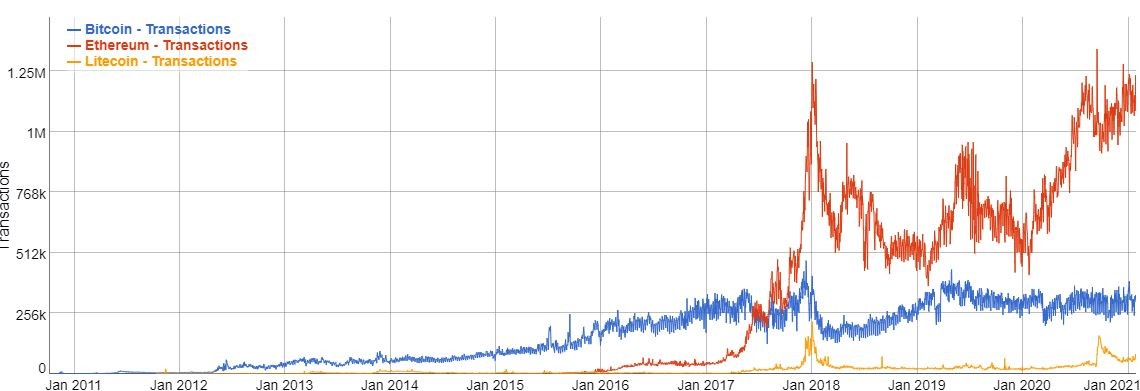
\includegraphics[scale=0.4]{assets/figures/blockchain_trend.jpg}
    \begin{flushleft}
        Quelle: Token S. 24
    \end{flushleft}
    \label{fig:birds8}
\end{figure}




Ist der Trend begründet und wird sich die Technologie durchsetzten?
\paragraph*{\mbox{}}
\textit{„This is an important time in the blockchain market as enterprises across markets and industries continue to increase their investment in the technology. The pandemic highlighted the need for more resilient, more transparent supply chains, healthcare delivery, financial services, and so much more, and enterprises around the world have been investing in blockchain to provide that resiliency and transparency,
    What is also very important right now is that we are seeing real interest and investment by corporations, financial institutions, and even governments in areas they previously viewed with some uncertainty such as cryptocurrencies, digital assets, central bank digital currencies, decentralized finance, and stablecoins. This investment will have major implications in a very short time on everything from retail to financial services to capital markets.“} \cite{Solutions}
\paragraph*{\mbox{}}
Dieses Zitat stammt von James Wester, Forschungsdirektor von Worldwide Blockschain Solutions. Laut ihm besteht kein Zweifel, dass Blockchainsysteme weiterhin wachsen und sich weiter entwickeln werden.
Belegt wird dieses Argument durch die jährlich steigenden Investitionen in Blockchain Solutions (siehe Abbildung unten).

\begin{figure}[!ht]
    \caption{Trend von Kryptowährungen}
    \includegraphics[scale=0.4]{assets/figures/investion blockchain solution.png}
    \begin{flushleft}
        Quelle: \url https://www.statista.com/statistics/800426/worldwide-blockchain-solutions-spending/
    \end{flushleft}
    \label{fig:birds7}
\end{figure}

Im Folgenden sollen nun beide Datenbanksysteme auf deren Wichtigste Kriterien untersucht werden.


\paragraphtitle{Kontrolle für Unternehmen}
Unternehmen benötigen einen bestimmten autoritativen Prozess, um die Blockchain-Technologie zu nutzen.
Anders als Big Data Anwendungen, werden öffentliche Blockchains nicht in der Lage sein, diese Kontrollmöglichkeiten in absehbarer Zeit zu bieten.
Der Aufstieg privater und konzerninterner Blockchains scheint jedoch sowohl die Kontrolle als auch den dezentralen Charakter der Technologie zu bieten.
Diese werden meist als Enterprise-Blockchain-Frameworks bezeichnet und sind nur für Organisationen geeignet.


\paragraphtitle{Sicherheit}
\textit{„Sicherheit ist kein Vorteil oder Upgrade. Man erreicht sie nicht, indem man neue Schichten aus Passwörtern hinzufügt.“} [1, Seite 22]
Durch ihre grundlegende Funktionsweise, Transaktionen und Daten auf vielen Rechnern eines Systems zu verteilen, hat die Verschlüsselung bei Blockchains einen hohen Stellenwert.
So würde beispielsweise der Angriff auf ein Bitcoin rund 30 Mrd. USD kosten.\cite{Bitcoin}
Dies geschieht durch Umschreibung der Information in eine anscheinend zufällige Abfolge von Zeichen. Dies geschieht durch den sogenannten Schlüssel, welcher erforderlich ist, um die Information zu decodieren.
Anders als bei der Blockchain, vertritt Big Data den umgekehrten Ansatz. Die Idee hinter Big Data ist, dass die frühere langsame, unbeholfene, schrittweise vorgehende Suche nach Wissen durch menschliche Gehirne ersetzt werden kann, wenn zwei Bedingungen zutreffen:
Alle Daten in der Welt können an einem einzigen Ort gesammelt werden und es können Algorithmen geschrieben werden, die hinreichend umfangreich sind, um sie zu analysieren.[1, Seite 35]
Hier besteht oftmals die Gefahr, dass, sollte besagter Server offline gehen oder sogar kompromitiert werden, die Web-Applikation nicht zuverlässig ist.

%\begin{figure}[!ht]
%    \caption{Manipulation des Ledgers}
%   \includegraphics[scale=1]{assets/figures/blockchange.png}
%    \begin{flushleft}
%       Quelle: Token S. 24
%    \end{flushleft}
%    \label{fig:birds2}
%\end{figure}


\paragraphtitle{Fälschungssicher}
Ein Versuch, einen Block in der Blockchain zu manipulieren, würde den Hashwert dieses Blockes ändern, da sich der Inhalt ändert. [3, Seite 100]
Der sogenannte Konsensmechanismus ist ein Programm, das die einzelnen Knotenpunkte innerhalb einer Blockchain vergleicht und in der Lage ist, legitime Transaktionen erst zu identifizieren und dann der Blockchain hinzuzufügen.
Grund hierfür ist die Tatsache, dass jeder einen Block zur Blockchain hinzufügen kann, weswegen sichergestellt werden muss, dass keine falschen Informationen zu Elementen der Blockchain werden.
Des Weiteren sorgt er dafür, dass es eine allgemeine Übereinkunft der Daten innerhalb des Blockchain-Netzwerkes gibt, so dass die Verlässlichkeit dieser Daten gewährleistet wird.

\paragraphtitle{Kontrolle}
Wie bereits in der Einleitung erwähnt, war einer der ausschlaggebendsten Elemente der Web 2.0-Epoche, dass die Nutzer auch die Rolle eines Produktes übernehmen.
Das zeigt sich beispielsweise an der Sammlung von Nutzerinformationen, welche dann genutzt werden, um für jeden Nutzer spezifische Werbungen zu schicken, je nach seinen Vorlieben.
Dies soll im Web 3.0 mit Hilfe von Blockchain von Grund auf anders aufgebaut werden. Stichwort Basic Attention Token, kurz BAT.
BAT ist ein System, welches in der Lage ist, die Aufmerksamkeit der Nutzer direkt zu belohnen.
Somit wird die Rolle aller Akteure der Onlinewerbebranche neu definiert, wie auch die Beziehung zwischen Nutzern, Publicer und Werbetreibenden.
Ziel dieser Idee ist, einen transparenteren und effizienteren Werbemarkt zu schaffen. BAT ist ein Token, welches von einer Public Blockchain verwaltet wird.
Der Brave Browser hat eine integrierte Wallet, die zwei Tokens verwaltet: BAT, welches als Zahlungsmittel verwendet wird, und Basic Attention Metrics, das sicherstellt, dass die Aufmerksamkeit der Nutzer genau gemessen und berichtet wird.
Werbetreibende senden diese BAT Tokens mitsamt den Werbeanzeigen verschlüsselt per Smart Contract. Sollte sich ein Nutzer dazu entscheiden, die Werbung anzusehen, kann er bis zu 70 Prozent der Werbeeinnahmen verdienen.
Der Rest geht an den Webseitenbetreiber.

\paragraphtitle{Anonymität}
Bei Web 2.0 Anwendungen findet die Nutzererkennung anhand der E-Mail-Adresse oder Benutzernamens zusätzlich des Passwortes statt.
Diese Informationen sind auf einem Server hinterlegt und werden geprüft, beispielsweise bei der Anmeldung.
Bei der Blockchain hingegen findet dies durch den Private Key statt, welcher auf einem P2P verschlüsselt hinterlegt ist.
Durch die hohe Verschlüsselung, sowie durch die hinter Private Keys versteckte Anonymität gelten Blockchain Datenbanksysteme als Möglichkeit, unbekannt im Netz zu agieren.
Dies hat sich bereits als reale Gefahr dargestellt, da viele illegale Aktivitäten, insbesondere im Zahlungsverfahren heutzutage über Kryptowährungen, wie typischerweise Bitcoin, ablaufen.
Insbesondere weil diese Zahlungen nicht nachverfolgbar sind.
\textit{„Der Betrag an Kryptowährung, der auf dem sogenannten Dark-Web-Marktplatz ausgegeben wurde, stieg in den letzten drei Monaten des Jahres 2019 um 60 Prozent auf einen neuen Höchststand von 601 Millionen US-Dollar, wie aus den am Dienstag veröffentlichten Daten von Chainalysis hervorgeht, einem Unternehmen, das alle Bitcoin-Transaktionen verfolgt und als Berater für mehrere Regierungsbehörden fungiert.} \cite{NewYorkTimes BlackMarket}

\begin{figure}[!ht]
    \caption{Bitcoin Wert im Darknet}
    \includegraphics[scale=0.7]{assets/figures/bitcoin_darkmarket.png}
    \begin{flushleft}
        Quelle: Token S. 19
    \end{flushleft}
    \label{fig:birds3}
\end{figure}

\paragraphtitle{Energieverbrauch}
Bei Big Data Netzwerken setzt sich der Energieverbrauch aus der durchgehenden Stromzufuhr des Servers und der des Kühlsystems zusammen, was zu hohen Energiekosten für das Unternehmen führt.
Bestimmte Blockchain-Konsensmechanismen haben jedoch höhere Energiekosten.
Wie bereits angemerkt muss ein Konsensprozess durchgeführt werden, um sicherzustellen, dass jede Transaktion gültig ist.
Es liegt auf der Hand, dass der Konsensprozess einen enormen Aufwand für die Bildung jedes Knotens erfordert.
Ganz zu schweigen davon, dass alle Knoten hin und her kommunizieren müssen, um sicherzustellen, dass eine Transaktion gültig ist.
Einige Blockchain-Netzwerke, wie beispielsweise Bitcoin, verwenden hierbei den Proof of Work, bei welchem jeder Node eine mathematische Funktion löst.
Der erste, der die Lösung der Funktion findet, bekommt als Belohnung Bitcoins.
Es gibt aber auch andere Konsensmechanismen, bei denen der Energieverbrauch deutlich geringer ist, so beispielsweise der Proof of Stake.
Anders als bei den Proof of Work, wird bei dem Proof of Stake gelost.
Der Gewinner, auch Validator genannt, überprüft den nächsten Block und alle darin aufgezeichneten Transaktionen.
Um an diesem Losverfahren teilzunehmen, müssen die Knoten, die als Validator fungieren wollen, eine bestimmte Anzahl von Coins in das Netz einbringen, was im Grunde als Garantie fungiert.
Je höher die Anzahl der Coins, der sogenannten Stake, desto höher ist die Wahrscheinlichkeit, als Validator ausgewählt zu werden.
Die als Garantie hinterlegten Coins garantieren auch, dass der Prüfer keine betrügerischen Transaktionen akzeptiert: tut er dies doch, verliert er einen Teil seines Stakes.
Als Belohnung für die Überprüfung erhält der Überprüfer in der Regel eine Transaktionsgebühr in Form eines Tokens des jeweiligen Netzwerkes.

\begin{figure}[!ht]
    \caption{Energieverbrauch PoW vs PoS}
    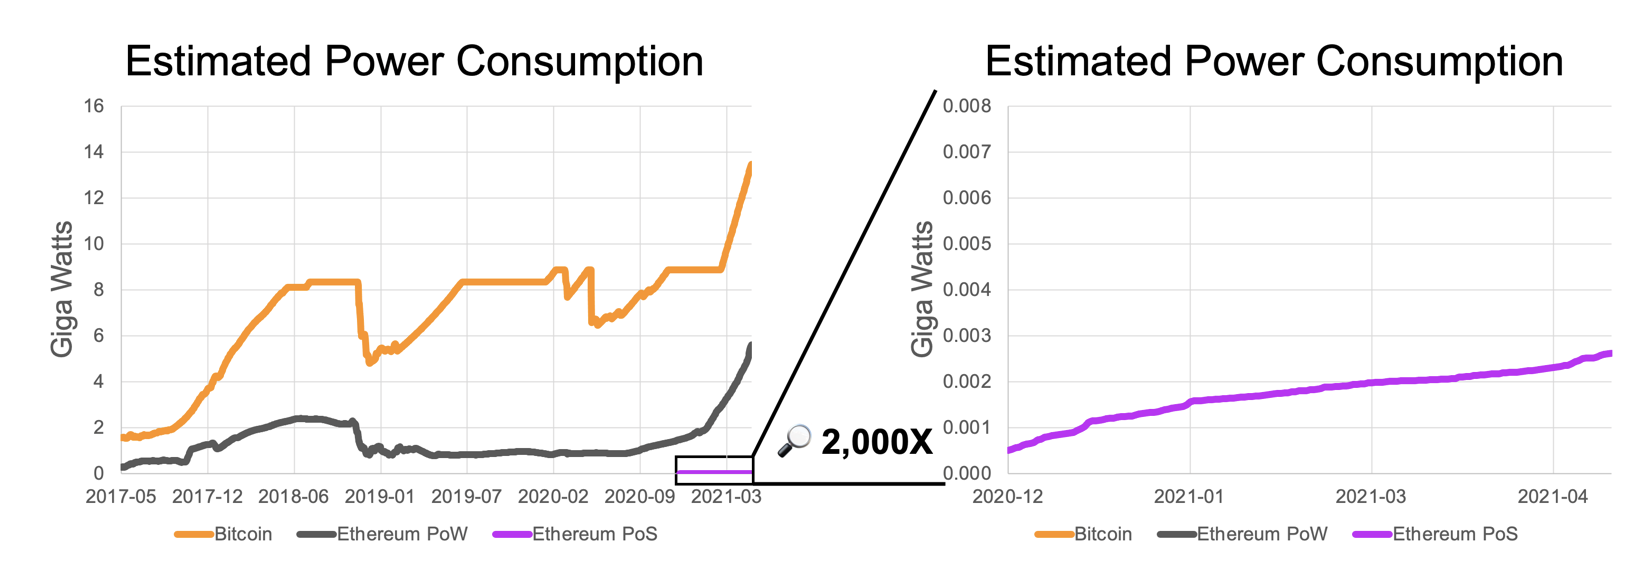
\includegraphics[scale=0.6]{assets/figures/power_consumption.jpg}
    \begin{flushleft}
        Quelle: Token S. 19
    \end{flushleft}
    \label{fig:birds4}
\end{figure}

\paragraphtitle{Kosten}
Zusätzlich zu den Energiekosten fallen noch weitere Gebühren an wie Hardware, Infrastruktur und Personal.
Bei einem dezentralen Netzwerk werden diese Dienstleistungen outsourced auf Freiwilligenbasis der Nutzer.

%FAZIT---------------------------------------------%
\subsection{Gründe für die Wahl der Hypothese}
Wie aus dem vorherigen Kapitel zu entnehmen ist, bieten sowohl Big Data als auch Blockchainsysteme viele verschiedene Vor- und Nachteile für Internetdienstleister.
Dezentrale Systeme haben die letzten Jahrzehnte stark geprägt und den Weg für viele neue Ideen und Systeme eröffnet.
Es gibt immer mehr Skandale in punkto Datenraub oder Intransparenz zentraler Webseitenbetreiber, was die allgemeine Nachfrage nach neuen, sichereren Alternativen steigen lässt.
Zusammen mit der sich verbessernden Technologien und den oben genannten Vorteilen lohnt es sich für viele Unternehmen, schon heute auf Blockchain umzusteigen.
Selbst wenn es ein eher langwieriger Prozess wird, wären vermutlich zehn Jahre ein denkbares Zeitfenster, um besagtes Ziel zu erreichen.


%FAZIT---------------------------------------------%
\subsection{Diskussion}


\subsubsection{Umsetzbarkeit}
Da die zugrundeliegende Technologie dafür schon gegeben ist, wäre die Frage vielmehr, ob sich die Umstellung für Unternehmen langfristig lohnt.
BitTorrent, Popcorn Time, BitMessage und Tor sind allesamt dezentrale Anwendungen, die von einem PHP-Netzwerk verwaltet werden, das kein Blockchain-Netzwerk ist.
Blockchain-Netzwerke sind eine verbesserte Form von P2P-Netzwerken.

\paragraphtitle{Public/Private Blockchain}
Der Unterschied zwischen einer Public und einer Private Blockchain liegt darin, wer Mitglied des Netzwerks sein und die Konsensmechanismen ausführen darf.
Jeder, der die im Protokoll festgelegten Regeln und Verfahren befolgt, kann einem öffentlichen Blockchain- Netzwerk  beitreten.
Bitcoin  zum  Beispiel  ist  ein öffentliches Blockchain-Netzwerk.
Im Gegensatz dazu ist ein privates Blockchain-Netzwerk geschlossen.
Private Netzwerke können nur per Einladung beigetreten werden.
Mitglieder müssen nach bestimmten Regeln validiert werden. Hier wird bestimmt, wer was sehen kann und wer an welchen Transaktionen teilnehmen darf.
Private Blockchains werden in der Regel von Unternehmen oder Regierungen betrieben, dabei können sich u. U. Einzelpersonen oder Organisationen daran beteiligen.

\paragraph*{\mbox{}}
Da außerdem die meisten Unternehmen bereits über ein zentrales Datenbanksystem verfügen, müssten sie für die entstehenden Kosten eines Wechsels aufkommen.
Man beachte hierbei, dass es aufgrund der Tatsache, dass die dazu erforderliche Technologie ein relativ wenig verbreitetes Konzept ist, nicht viele fähige Entwickler gibt, die daran arbeiten können.
Wenn Unternehmen also versuchen, ihre Blockchain-Lösung für den eigenen Betrieb zu entwickeln, kann es u. U. schwierig werden, ein fähiges Team fürs Projekt zu finden.
Blockchain ist nicht für Unternehmen gedacht, die Legacy-Netzwerke (ältere Systeme) betreiben.
In Wirklichkeit würde die Blockchain die alten Netze ersetzen.
Allerdings ist der Integrationsprozess noch nicht voll funktionsfähig.
Außerdem sind viele Blockchain-Technologien nicht in der Lage, mit den alten Netzen zusammenzuarbeiten.
Das bedeutet, dass die Unternehmen, um sie richtig nutzen zu können, ihre alten Netze endgültig abschaffen müssten.
Diesem Umstand stehen viele skeptisch gegenüber.


\subsubsection{Zukunftstauglichkeit}
Das Internet hat sich in den letzten Jahren zu einem Einkaufsladen für Benutzerinformationen verwandelt, von welchem die Nutzer kaum profitieren.
P2P-Netzwerke wie Blockchain versprechen hier Anonymität, Kontrolle und Sicherheit und vor allem weniger Abhängigkeit von Unternehmen.

\textit{„Wir überschätzen immer die Veränderungen, die in den nächsten beiden Jahren passieren sollen. Aber wir unterschätzen den Wandel, der über die nächsten zehn Jahre passiert. Lass dich dadurch nicht zur Untätigkeit verleiten.“} - Bill Gates [3, Seite 46]

Wie bereits festgestellt existiert bereits eine vielversprechende Technologie dazu.
Im letzten Jahrzehnt kam es zu hunderten Skandalen von Big-Data-Unternehmen aufgrund ihrer teilweise fragwürdigen Strategien, Profit zu erzielen.
Auf Blockchain basierende Seiten bieten hingegen eine höhere Transparenz, sowie die Möglichkeit für Nutzer, sich an diesem Prozess finanziell selbst zu bereichern.
Auch wenn die Technologie von Blockchain Netzwerken und der gesetzliche Rahmen dazu noch nicht ausgereift ist, besagt der Trend, dass wir damit zu rechnen haben, zumal es bereits funktionierende Geschäftsmodelle und Währungen gibt.
Viele Tech-Führungskräfte und Ingenieure haben bereits große IT-Unternehmen wie Google, Meta und Amazon verlassen, um die ihrer Meinung nach einmalige Chance der Kryptowährung zu nutzen.\cite{NewYorkTimes StartUp}
%FAZIT---------------------------------------------%
\subsection{Fazit}
Auch wenn wir uns mittlerweile auf die Zuverlässigkeit unzähliger Dienste verlassen, laufen im Hintergrund Datenbanken, welche im Kern wenig Sicherheit gewährleisten können.
Unberechtigte Zugriffe sind möglich und können nicht immer verfolgt werden. DLTs ändern das, und so sind sie denkbar eine Technologie fürs kommende Zeitalter.
Verschlüsselung, Speicherung, Validierung und Sicherung der Daten funktionieren hier in einer integrierten Lösung.
Alle Daten, denen wir vertrauen müssen, werden in Zukunft in einem Distributed Ledger bzw. einer Blockchain gespeichert werden. Neue Geschäftsmodelle können entstehen – direkt zwischen Nutzern und Anbietern, ohne Mittelsmänner.
Es ist allerdings auch zu bedenken, dass herkömmliche Datenbanken deutlich effizienter, einfacher und günstiger zu betreiben sind.
Überall dort, wo wir die Sicherheit der Blockchain oder Funktionen wie Smart Contracts nicht brauchen, sind sie daher weiterhin die bessere Wahl.

%FAZIT---------------------------------------------%
\subsection{Verifikation der Hypothese}
Bei der Überprüfung dieser These, ist festzustellen, dass auch wenn der genaue Zeitramen ungewiss ist, so scheint der allgemeine Trend, sowie die vielversprechenden Vorteile, welche die Blockchain Struktur zu bieten haben, darauf hinzudeuten, dass mit an sicherheit grenzender Wahrscheinlichkeit sich diese bewahrheiten wird.
\chapter{Schluss}

Lorem ipsum dolor sit amet\footnote{Vgl. Baumann, M. F. u. a., Taking responsibility: A responsible research and innovation (RRI) perspective on insurance issues of semi-autonomous driving, 2019, S. 558.}, consetetur sadipscing elitr, sed diam nonumy eirmod tempor invidunt ut labore et dolore magna aliquyam erat, sed diam voluptua.
At vero eos et accusam et justo duo dolores et ea rebum.
Stet clita kasd gubergren, no sea takimata sanctus est Lorem ipsum dolor sit amet.
Automation in cars has a long history.  Lorem ipsum dolor sit amet, consetetur sadipscing elitr, sed diam nonumy eirmod tempor invidunt ut labore et dolore magna aliquyam erat, sed diam voluptua.
At vero eos et accusam et justo duo dolores et ea rebum.
Stet clita kasd gubergren, no sea takimata sanctus est Lorem ipsum dolor sit amet Acceptance of autonomous driving will depend on how far a consensus on these norms can be found, first among experts, then in society at large.
One ethical condition, however, should be crucial: in no case should the ethical algorithms be put in practice as nontransparent black boxes.
The built-in norms should, as far as possible, be understood and commonly shared.

\section{Kurzzusammenfassung der Arbeit}

Lorem ipsum dolor sit amet, consetetur sadipscing elitr, sed diam nonumy eirmod tempor invidunt ut labore et dolore magna aliquyam erat, sed diam voluptua.
At vero eos et accusam et justo duo dolores et ea rebum.
Stet clita kasd gubergren, no sea takimata sanctus est Lorem ipsum dolor sit amet.
Automation in cars has a long history.  Lorem ipsum dolor sit amet, consetetur sadipscing elitr, sed diam nonumy eirmod tempor\footnote{Vgl. Baumann, M. F. u. a., Taking responsibility: A responsible research and innovation (RRI) perspective on insurance issues of semi-autonomous driving, 2019, S. 558.} invidunt ut labore et dolore magna aliquyam erat, sed diam voluptua.
At vero eos et accusam et justo duo dolores et ea rebum.
Stet clita kasd gubergren, no sea takimata sanctus est Lorem ipsum dolor sit amet Acceptance of autonomous driving will depend on how far a consensus on these norms can be found, first among experts, then in society at large.
One ethical condition, however, should be crucial: in no case should the ethical algorithms be put in practice as nontransparent black boxes.
The built-in norms should, as far as possible, be understood and commonly shared.

\section{Weitere Empfehlungen}

Lorem ipsum dolor sit amet, consetetur sadipscing elitr, sed diam nonumy eirmod tempor invidunt ut labore et dolore magna aliquyam erat, sed diam voluptua.
At vero eos et accusam et justo duo dolores et ea rebum.
Stet clita kasd gubergren, no sea takimata sanctus est Lorem ipsum dolor sit amet.
Automation in cars has a long history.  Lorem ipsum dolor sit amet, consetetur sadipscing elitr, sed diam nonumy eirmod tempor invidunt ut labore et dolore magna aliquyam erat, sed diam voluptua.
At vero eos et accusam et justo duo dolores et ea rebum.
Stet clita kasd gubergren, no sea takimata sanctus est Lorem ipsum dolor sit amet Acceptance of autonomous driving will depend on how far a consensus on these norms can be found, first among experts, then in society at large\footnote{Vgl. Baumann, M. F. u. a., Taking responsibility: A responsible research and innovation (RRI) perspective on insurance issues of semi-autonomous driving, 2019, S. 558.}.
One ethical condition, however, should be crucial: in no case should the ethical algorithms be put in practice as nontransparent black boxes.
The built-in norms should, as far as possible, be understood and commonly shared.



%end of document
\end{document}